\documentclass{article}

\usepackage{tikz}
	\usetikzlibrary{positioning,fit,calc, decorations, arrows, shapes, shapes.geometric}
	\usetikzlibrary{cd}

	%%%%%%%%%%%%
	\tikzset{AmpRep/.style={ampersand replacement=\&}}
	\tikzset{center base/.style={baseline={([yshift=-.8ex]current bounding box.center)}}}
	\tikzset{paperfig/.style={center base,scale=0.9, every node/.style={transform shape}}}

	% Node Stylings
	\tikzset{dpadded/.style={rounded corners=2, inner sep=0.7em, draw, outer sep=0.3em, fill={black!50}, fill opacity=0.08, text opacity=1}}
	\tikzset{dpad0/.style={outer sep=0.05em, inner sep=0.3em, draw=gray!75, rounded corners=4, fill=black!08, fill opacity=1}}
	\tikzset{dpad/.style args={#1}{every matrix/.append style={nodes={dpadded, #1}}}}
	\tikzset{light pad/.style={outer sep=0.2em, inner sep=0.5em, draw=gray!50}}

	\tikzset{arr/.style={draw, ->, thick, shorten <=3pt, shorten >=3pt}}
	\tikzset{arr0/.style={draw, ->, thick, shorten <=0pt, shorten >=0pt}}
	\tikzset{arr1/.style={draw, ->, thick, shorten <=1pt, shorten >=1pt}}
	\tikzset{arr2/.style={draw, ->, thick, shorten <=2pt, shorten >=2pt}}

\usepackage[utf8]{inputenc}
\usepackage{mathtools}
% \usepackage{bbold}
\usepackage{amssymb, graphicx}
\usepackage{parskip}
\usepackage{algorithm}
\usepackage{bbm}
% \usepackage{algpseudocode}
\usepackage{graphicx}
\usepackage[margin=1in]{geometry}
\usepackage{scalerel}

\usepackage{hyperref} % Load before theorems...


\usepackage{enumitem}
\usepackage{amsthm,thmtools}
	\usepackage[noabbrev,nameinlink,capitalize]{cleveref}
    \theoremstyle{plain}
    \newtheorem{theorem}{Theorem}
	\newtheorem{coro}{Corollary}[theorem]
    \newtheorem{prop}[theorem]{Proposition}
    \newtheorem{claim}{Claim}
    \newtheorem{remark}{Remark}
    \newtheorem{lemma}[theorem]{Lemma}
    \theoremstyle{definition}
    \declaretheorem[name=Definition, qed=$\square$]{defn}

	\crefname{defn}{Definition}{Definitions}
	\crefname{prop}{Proposition}{Propositions}

\usepackage{nicefrac}\let\nf\nicefrac
\usepackage{color}
%\usepackage{stmaryrd}
\hypersetup{colorlinks=true, linkcolor=blue!75!black, urlcolor=magenta, citecolor=green!50!black}

\relax %%%%%%%%% GENERALL MACROS %%%%%%%%
    \let\Horig\H
	\let\H\relax
	\DeclareMathOperator{\H}{\mathrm{H}} % Entropy
	\DeclareMathOperator{\I}{\mathrm{I}} % Information
	\DeclareMathOperator*{\Ex}{\mathbb{E}} % Expectation

    \newcommand{\mat}[1]{\mathbf{#1}}
    \DeclarePairedDelimiterX{\infdivx}[2]{(}{)}{%
		#1\;\delimsize\|\;#2%
	}
	\newcommand{\thickD}{I\mkern-8muD}
	\newcommand{\kldiv}{\thickD\infdivx}
	\newcommand{\tto}{\rightarrow\mathrel{\mspace{-15mu}}\rightarrow}

	\newcommand{\datadist}[1]{\Pr\nolimits_{#1}}
	% \newcommand{\datadist}[1]{p_\text{data}}


\relax %%%%%%%%%   PDG  MACROS   %%%%%%%%
	\newcommand{\bp}[1][L]{\mat{p}_{\!_{#1}\!}}
	\newcommand{\V}{\mathcal V}
	\newcommand{\N}{\mathcal N}
	\newcommand{\Ed}{\mathcal E}

	\DeclareMathAlphabet{\mathdcal}{U}{dutchcal}{m}{n}
	\DeclareMathAlphabet{\mathbdcal}{U}{dutchcal}{b}{n}
	\newcommand{\dg}[1]{\mathbdcal{#1}}

	\newcommand\Inc{\mathit{Inc}}
	\newcommand{\IDef}[1]{\mathit{IDef}_{\!#1}}
	\newcommand{\ed}[3]{%
		\mathchoice%
		{#2\overset{\smash{\mskip-5mu\raisebox{-3pt}{${#1}$}}}{\xrightarrow{\hphantom{\scriptstyle {#1}}}} #3} %display style
		{#2\overset{\smash{\mskip-5mu\raisebox{-3pt}{$\scriptstyle {#1}$}}}{\xrightarrow{\hphantom{\scriptstyle {#1}}}} #3}% text style
		{#2\overset{\smash{\mskip-5mu\raisebox{-3pt}{$\scriptscriptstyle {#1}$}}}{\xrightarrow{\hphantom{\scriptscriptstyle {#1}}}} #3} %script style
		{#2\overset{\smash{\mskip-5mu\raisebox{-3pt}{$\scriptscriptstyle {#1}$}}}{\xrightarrow{\hphantom{\scriptscriptstyle {#1}}}} #3}} %scriptscriptstyle

    \newcommand{\nhphantom}[2]{\sbox0{\kern-2\nulldelimiterspace$\left.\delimsize#1\vphantom{#2}\right.$}\hspace{-.97\wd0}}
	\newcommand\DeclareDoubleDelim[5]{
	    \DeclarePairedDelimiterX{#1}[1]{#2}{#5}
		    {\nhphantom{#3}{##1}\hspace{1.2pt}\delimsize#3\mathopen{}##1\mathclose{}\delimsize#4\hspace{1.2pt}\nhphantom{#4}{##1}}
	}
	\DeclareDoubleDelim
		\SD\{\{\}\}
	\DeclareDoubleDelim
		\bbr[[]]
	% \DeclareDoubleDelim
	% 	\aar\langle\langle\rangle\rangle
	\makeatletter
	\newcommand\aar{\@ifstar\aar@resize\aar@plain}
	\newcommand\aar@resize[1]{\scaleleftright[3.8ex]{\Biggl\langle\!\!\!\!\Biggl\langle}{#1}
		{\Biggr\rangle\!\!\!\!\Biggr\rangle}}
	\DeclareDoubleDelim
		\aar@plain\langle\langle\rangle\rangle
	\makeatother
	% \DeclarePairedDelimiterX{\aar}[1]{\langle}{\rangle}
	% 	{\nhphantom{\langle}{#1}\hspace{1.2pt}\delimsize\langle\mathopen{}#1\mathclose{}\delimsize\rangle\hspace{1.2pt}\nhphantom{\rangle}{#1}}

\newcommand\todo{\textcolor{red}{Todo: }}


\title{PDG Inconsistency: The Universal Loss}
\date{May 2021}

\allowdisplaybreaks


\begin{document}

\maketitle


\begin{abstract}
	Probabilistic Dependency Graphs (PDGs) are a general class of graphical model, which can incorporate arbitrary---even inconsistent---conditional probabilistic information, weighted by confidence.

	This ability to capture inconsitency was originally intended to capture fallable agents,
	but here we show that it is also valuable for capturing trainable models.
	For example, a variational autoencoder (VaE)
	has three pieces of probablistic information: an encoder $e(Z \mid X)$, a decoder $d(X \mid Z)$, and a prior $p(Z)$. In general, there will be no joint distribution $\Pr(X,Z)$ that matches all three, so if specified by neural network weights, they will likely be inconsistent. Training can be viewed as the process of updating them so that they are consistent with one another and also observations of $X$.
	Surprisingly, the inconsistency of a PDG containing $p,d,e$ and a sample $x$ is precisely $\mathit{ELBO}_{p,d,e}(x)$, the objective usually used to train VaEs.

	More broadly, we show that PDG inconsistency generates many natural loss functions functions, and suggest that some relationships between them---such as variational bounds---can be justified in an more intuitive manner via the relationships of their underlying PDG.
\end{abstract}

\section{Introduction}
% -universality
Many tasks in artificial intelligence can be fruitfully cast as optimization problems, but often the choice of objective is not unique.
For instance, a loss function is a key component of a machine learning system, but hinge loss, cross entropy, and mean squared error are all popular loss functions motivated by similar intuitions of `distance to ground truth', drawing from different formalisms.
Each implicitly represents different values, and results in different behavior, and so this choice can be quite important---and yet because the crieteria for choosing a ``good'' loss function are often inscrutible, it is often made arbitrarily.
Furthermore, there is often something to be gained by fiddling with these loss functions: one can add regularization terms, to incentivize desirable behavior.
But the process of tinkering with the objective to get desirable behavior, and afterwards spinning a story about why it works, leaves something to be desired:
the tinkering itself can be a tedious game without well-defined rules, while results so obtained are vulnerable to overfitting and pedagogically difficult to motivate.
%
% We attribute this state of affairs to the relative permisiveness of the medium of expression.
% ...


By contrast, a choice of \emph{model} admits more principled discussion, in part because it makes sense to ask if a model is accurate, or of it captures some intuition about reality.
This observation motivates our proposition: the use of model inconsistency a ``universal'' loss function. In this framework, it is no longer possible to specify an objective directly; rather, one must articulate a situation that gives rise to it, in the (more interpretable) language of probablistic beliefs and certainties. % (concretely, as a PDG \cite{richardson2020probabilistic}).
Concretely, we use the machinery Probabilistic Dependency Graphs (PDGs), a particularly expressive class graphical models which can can incorporate aribtrary (even inconsistent) probabilistic information in a natural way, and comes equipped with a well-motivated information-theoretic measure of inconsistency  \cite{richardson2020probabilistic}.
Not all mathematical formulas can be expressed in this way,
but surprisingly, most standard objective functions (such as cross entropy, KL divergence, Bhattacharyya distance, reny\'i entropies, the ELBO, L1 and L2 regularizers, log partition functions) arise naturally as inconsistencies of the appropriate underlying PDG.
% which surprised us because it was not designed with any of them in mind, but rather from purely information-theoretic considerations.
As a result, such a scheme of objective specification is more restrictive, but also more intuitive (since knowledge of the objectives listed above is not necessary), and admits more epistemically grounded support and criticism.
This change is analogous to a higher-level programming language, which restricts the set of legal programs but makes them easier to reason about, and ultimately, even easier to write.


Representing objectives as model inconsistencies, in addition to providing a principled way of selecting an objective, also has beneficial pedagogical side effects.  For instance, the relationships between the underlying models give rise to very simple and intuitive proofs of otherwise opaque inequalities, such as the variational bounds, and of the Reny\'i entropy's monotonicity in its parameter $\alpha$.


% Is there a deeper reason to use one measure of  these terms?

% % This state of affairs presents some problems. One is scientific.
% Another is pedagogical. Where does cross-entropy come from? What about the ELBO?


In the coming sections, we will show how this concept of inconsistency, beyond simply providing a forgiving and intuitive modeling framework, reduces exactly to many standard objectives used in machine learning, and also demonstrate that this framework clarifies the relationships between them, by providing simple clear derivations of otherwise opaque inequalities.


\subsection{Related Work}

This approach naturally extends work in the Bayesian ML community%
%TODO: find a real academic reference for this material.
\footnote{\url{https://towardsdatascience.com/a-bayesian-take-on-model-regularization-9356116b6457}}
establishing a correspondence between regularizers and priors.
We note that a primary benefit of this correspondance is the ability to view (some) regularizers as \emph{prior beliefs}, which are modeling assumptions.


In parallel work on inference on inference with PDGs, we show that many standard algorithms for inference in other probablisitc models can be viewed as algorithms for reducing inconsistency of the relevant PDG.


\section{Preliminaries}
% Method: What machine learning techniques are you planning to apply or improve upon and how? Make sure to describe them in detail and provide enough context for the reader to understand the methods at least at a high level. Provide any background that is necessary for that.
A PDG, like a Bayesian Network (BN), is a directed graph, to which we attatch a conditional probability distributions (cpds). While this data is attached to the \emph{nodes} of a BN, it is attached to the \emph{edges} of PDG.
Concretely, in a BN, the variable $X$ is associated with the distribution $\bp[X](X \mid \mathbf{Pa}(X))$ on $X$ given its parents; an edge $X \to Y$ is associated with a distribution $\bp(Y \mid X)$.
As a result, a PDG of shape $X \to Y \rightarrow Z$ describes a distributon on $Y$ given $X$ and also a distribution on $Y$ given $Z$, while it describes a joint dependence in a BN.
Although it won't play a large role here, it is worth noting that, the PDG interpretation is more general and can capture joint as well.
Formally, the syntax of a PDG is given in \cref{defn:pdg}, but beforehand let's quickly fix some notation for use in the rest of the paper.

We use capital letters for variables, and lower case letters for their values.
Depending on which is clearer in context, we write either $\Ex_\mu X$ or $\Ex_{\omega \sim \mu} X(\omega)$ for expectation of a random variable $S$ over a distribution $\mu$, with outcomes $\Omega$.
$\H(\mu)$ and $\H_\mu(X)$, $\H_\mu(Y \mid X)$ refer respectively to the entropy of a distribution $\mu$, the entropy of the variable $X$ with respect to $\mu$, and the conditional entropy of $Y$ given $X$, with respect to $\mu$. We are now read to present the definition.

\begin{defn}\label{defn:pdg}
	A Probabilistic Dependency Graph (PDG) is a tuple $\dg M = (\N,\Ed,\V,\mat p, \alpha, \beta)$ , where
	\begin{description}[leftmargin=1em,labelindent=1.5em,itemsep=0pt]
		\item[$\N$]
			is a finite set of nodes, corresponding to variables;
		\item[$\Ed$]
			is a set of labeled  (hyper)-edges $\{ \ed LXY \}$, each with a source
			$X$ and target $Y$ in $\N$;
		\item[$\V$]
			associates each variable $N \in \N$ with a set $\V(N)$ of values that the variable $N$ can take;
		\item[$\mat p$]
		associates to each edge $\ed LXY \in \Ed$
		a distribution $\bp(x)$ on $Y$ for each $x \in \V(X)$;
	\item[$\alpha$]
	associates to each edge $\ed LXY$ a non-negative number $\alpha_L$ which,
	roughly speaking, is the modeler's confidence in the functional
	dependence of $Y$ on $X$ implicit in $L$;
	\item[$\beta$]
	associates to each edge $L$ a real number $\beta_L$,
	the modeler's subjective confidence in the reliability of
	$\bp$.
	\end{description}
\end{defn}

This presentation is equivalent to one in which edges are litterally directed hyper-edges, that have sets of variables as sources and targets.
An unconditional distribution $p(X)$ can be given by associating it to a hyper-edge $\emptyset \to \{X\}$, or directly by \cref{defn:pdg} by taking its source to be a variable with only one value.
% We will not make much use of $\alpha$ here, so $\mat p$ and $\beta$ are the most important

PDGs, like other graphical models, have semantics in terms of joint distributions over all variables.
Most directly, a PDG $\dg M$ determines a family of loss (scoring) functions on joint distributions $\mu$, with a single parameter $\gamma > 0$, given by
\begin{equation}
	\bbr{\dg M}_\gamma(\mu) = \gamma \IDef{\dg M}(\mu) +  \sum_{\ed LXY} \Ex_{x \sim \mu(X)} \beta_L \kldiv[\Big]{\mu(Y\mid x)}{\bp(Y \mid x)}
	\label{eq:semantics}
\end{equation}
where $\kldiv\mu\nu$ is the relative entropy (KL Divergence) of $\nu$ with respect to $\nu$, and $\IDef{\dg M}(\mu) = - \H(\mu) + \sum_{\ed LXY} \alpha_L \H(Y \mid X)$, called the information deficiency, plays a minimal role in the present context, but measures the degree to which $\mu$ reflects the qualitative features one would expect if it were generated by the causal weighted graph $(\N, \Ed, \alpha)$.
We assert that for the examples here, we can select $\alpha$ such that $\IDef{\dg M}(\mu) = 0$ for all $\mu$, and we can also set $\gamma=0$ to ignore it explicitly.
The remaining terms of \eqref{eq:semantics} serve to assign a candidate distribution $\mu$ a larger cost if its associated conditional marginals deviate more from the cpds in the PDG, and especially so for the cpds with high confidence.

The \emph{best} distribution by this metric (the one with the smallest loss), denoted $\bbr{\dg M}^*$
% = \arg\min_\mu \bbr{\dg M}(\mu)$
 exists and is unique for small enough $\gamma$, and in the limit as $\gamma \to 0$; we interpret it in this limit ($\gamma \to 0$) when no subscript is supplied.
 The \emph{inconsistency} of $\dg M$ is the minimum value attained by the loss function, for any $\mu$, and is denoted by $\aar{\dg M}_\gamma$. Because we will not be playing with the qualitative half, we will generally drop the subscript $\gamma$; the results can be interpretd directly for $\gamma = 0$, and can be extended for all others values as well, with careful choice of $\alpha$.
 % := \inf_\mu \bbr{\dg M}(\mu)$.


 	A cpd $p$ can be regarded as a PDG with a single edge, and sometimes we will implicitly convert a cpd to a PDG.
	The union of $\dg M$ and $\dg M'$ is denoted by $\dg M + \dg M'$.
	A value $x$ of a variable $X$ is identified with the degenerate distribution $\delta_x$ that places all mass on $x$, and hence may be associated to an edge.
 	By default, all cpds are associated with confidence $\beta = 1$, unless specified otherwise, which will be done as a parameter list over the name of the cpd, as in $\overset{(\beta:0.7)}p$. We will use an exclamation point (e.g., $\ed {p!}XY$) to inciate the limit of high confidence ($\beta_p \to \infty$).

It is easy to show that adding edges, or increasing their confidences, cannot decrease the inconsistency of a PDG.
Intuitively, believing more things can't make you any less inconsistent.
This is captured formally in two different (but related) ways by the following lemma, which is the primary tool we will use to derrive relationships between loss functions.
\begin{lemma}[addopting beliefs cannot decrease inconsistency]\label{lemma!}

	\begin{enumerate}
		\item For all pdgs $\dg M$, $\dg M'$, we have that  $\aar{\dg M + \dg M'} \ge \aar{\dg M}$.
		\item If $\dg M$ and $\dg M'$ have respective confdience vectors $\beta$ and $\beta'$, and $\beta \succeq \beta'$ (that is, $\beta_L \ge \beta'_L$ for all $L \in \Ed$), then $\aar{\dg M} \ge \aar{\dg M'}$.
	\end{enumerate}

\end{lemma}
\begin{proof}
	For every $\mu$, adding more edges only adds non-negative terms to \eqref{eq:semantics}.
	In the first case this means, $\bbr{\dg M + \dg M'}_\gamma(\mu) \ge \bbr{\dg M}_\gamma(\mu)$ for all $\gamma$ and $\mu$. So it also holds when we take an infemum over $\mu$, giving $\aar{\dg M + \dg M'}_\gamma \ge \aar{\dg M}_\gamma$. Analogously, increasing $\beta$ results in larger scalings for non-negative terms in \eqref{eq:semantics} so $\bbr{\dg M}_\gamma(\mu) \ge \bbr{\dg M'}_\gamma(\mu)$ for all $\gamma$ and $\mu$.
\end{proof}


\section{Simple Information-Theoretic Objectives as Inconsistency}
\def\xsamp{{\underline{\mat x}}}
\def\xysamp{{\underline{\mat{xy}}}}

To illustrate how the inconsistency of a PDG can start to generate information theoretic expressions, let's start with a simple example. Suppose you believe that $X$ is distributed according to $p$, and also that it (always) equals a certain value $x$. These beliefs are entirely consistent if $p(X=x) = 1$, and become more inconsistent as $p(X = x)$ drops. In fact, it is equal to the surprise of seeing $x$ or the information content of $X = x$, according to $p$.

\begin{prop}\label{prop:pdg-Ix}
	Consider a distribution $p(X)$.
	The surprise $\I_p(x)$ at seeing a sample $x$ is given by the inconsistency of the pdg containing a point mass on $x$ and $p$, i.e.,
	\[\I_p(x) := \log \frac{1}{p(x)} =
	\aar[\Big] {
	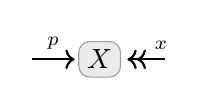
\begin{tikzpicture}[center base]
		\node[dpad0] (X) {$X$};
		\coordinate (A) at ($(X) + (-0.9,0)$);
		\draw[arr1] (A) -- node[above]{$\scriptstyle p$}  (X);
%
		\draw[arr2, <<-] (X) --  node[above,pos=0.8]{$\scriptstyle x$} ++(0.9, 0);
	\end{tikzpicture}
	}.
	\]
\end{prop}
\begin{proof}
	Any distribution $\mu(X)$ that places mass on some $x' \ne x$ will have infinite KL divergence from the point mass on $x$. Thus, the only possibility for a finite consistency arises when $\mu = \delta_x$, and so
	\begin{equation*}
		\aar[\Big] {
		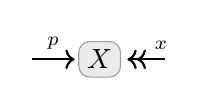
\begin{tikzpicture}[center base]
			\node[dpad0] (X) {$X$};
			\coordinate (A) at ($(X) + (-0.9,0)$);
			\draw[arr1] (A) -- node[above]{$\scriptstyle p$}  (X);
	%
			\draw[arr2, <<-] (X) --  node[above,pos=0.8]{$\scriptstyle x$} ++(0.9, 0);
		\end{tikzpicture}
		}
		= \bbr*{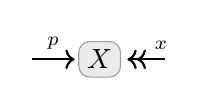
\begin{tikzpicture}[center base]
			\node[dpad0] (X) {$X$};
			\coordinate (A) at ($(X) + (-0.9,0)$);
			\draw[arr1] (A) -- node[above]{$\scriptstyle p$}  (X);
	%
			\draw[arr2, <<-] (X) --  node[above,pos=0.8]{$\scriptstyle x$} ++(0.9, 0);
		\end{tikzpicture}}( \delta_x )
		= \kldiv{\delta_x}{p} = \log \frac{1}{p(x)} = \I_p(x).
	\end{equation*}
\end{proof}

The value $\I_p(x) = -\log p(x)$ also goes by the name ``negative log likelihood'', and is most common objective for training generative models, corresponding to ``maximizing the probability of seeing your data''.
\Cref{prop:marginal-ll,prop:many-equal-simple} generalize this result in two different directions. First, the inconsistency is localized to $x$, where the sample conflicts with the distribution; other variables don't make a difference.

\begin{prop} \label{prop:marginal-ll}
	If $p(X,Z)$ is a joint distribution, the information content of the partial observation $X=x$, or the marginal negative log likelihood of $x$, is given by
	\[\displaystyle \I_p(x) = \log \frac{1}{p(x)} =
	    % \lim_{t \to \infty}
		 \aar[\Bigg]{
	% 	  \Inc\left(
			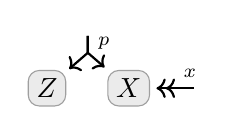
\begin{tikzpicture}[center base]
				\node[dpad0] (Z) {$Z$};
				\node[dpad0,right=.5 of Z] (X) {$X$};
				\coordinate (A) at ($ (X)!.5!(Z) + (0,0.7)$);
				\draw[arr1] (A) -- node[right]{$\scriptstyle p$} ++(0,-0.25) -- (X);
				\draw[arr1] (A) -- ++(0,-0.25) -- (Z);
	%
				\draw[arr2, <<-] (X) --  node[above,pos=0.8]{$\scriptstyle x$} ++(0.9, 0);
	% 			\draw[arr2, <-] (Z) -- node[above,pos=0.6]{$\scriptstyle q^{\{\beta =\infty\}}$} ++(-0.9, 0);%
				% \ar[r,"p"] \& Z \ar[r,"p", bend left] \& X \ar[l,"q", bend left] \& \ar[l, two heads, "x"']
			\end{tikzpicture}
			}. \]
\end{prop}
\begin{proof}
	As before, all mass of $\mu$ must be on $x$ for it to have a finite score.
	Thus it suffices to consider joint distributions of the form $\mu(X,Z) = \delta_x(X) \mu(Z)$.
	We have
	\begin{align*}
	\aar*{
		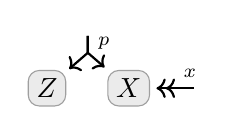
\begin{tikzpicture}[center base]
			\node[dpad0] (Z) {$Z$};
			\node[dpad0,right=.5 of Z] (X) {$X$};
			\coordinate (A) at ($ (X)!.5!(Z) + (0,0.7)$);
			\draw[arr1] (A) -- node[right]{$\scriptstyle p$} ++(0,-0.25) -- (X);
			\draw[arr1] (A) -- ++(0,-0.25) -- (Z);
			\draw[arr2, <<-] (X) --  node[above,pos=0.8]{$\scriptstyle x$} ++(0.9, 0);
		\end{tikzpicture}}
			&= \inf_{\mu(Z)} \bbr*{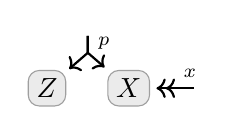
\begin{tikzpicture}[center base]
				\node[dpad0] (Z) {$Z$};
				\node[dpad0,right=.5 of Z] (X) {$X$};
				\coordinate (A) at ($ (X)!.5!(Z) + (0,0.7)$);
				\draw[arr1] (A) -- node[right]{$\scriptstyle p$} ++(0,-0.25) -- (X);
				\draw[arr1] (A) -- ++(0,-0.25) -- (Z);
				\draw[arr2, <<-] (X) --  node[above,pos=0.8]{$\scriptstyle x$} ++(0.9, 0);
			\end{tikzpicture}}\Big(\delta_x(X)\mu(Z)\Big)  \\
			&= \inf_{\mu(Z)}\kldiv[\Big]{\delta_x(X)\mu(Z)}{p(X,Z)} \\
			&= \inf_{\mu(Z)}\Ex_{z \sim \mu} \log \frac{\mu(z)}{p(x,z)}
			~= \inf_{\mu(Z)}\Ex_{z \sim \mu} \log \frac{\mu(z)}{p(x,z)}\frac{p(x)}{p(x)} \\
			&= \inf_{\mu(Z)}\Ex_{z \sim \mu} \left[ \log \frac{\mu(z)}{p(z \mid x)} + \log \frac{1}{p(x)} \right] \\
			&= \inf_{\mu(Z)} \Big[\kldiv{\mu(Z)}{p(Z\mid x)}\Big] + \log \frac{1}{p(x)} \\
			&= \log \frac{1}{p(x)} = \I_p(x) & \text{[Gibbs Inequality]}
	\end{align*}
\end{proof}


Of course, we usually have more than one sample. In this case, we have a more sophisticated data distribution. The first step in the proof of \cref{prop:pdg-Ix} no longer works, but we can get the same effect by increasing confidence in the data distribution.

\begin{prop} \label{prop:many-equal-simple}
	Given samples $\xsamp = \{ x_i \}_{i=1}^m$ determining an emperical distribution $\datadist\xsamp$,  the following are equal, for all $\gamma \ge 0$:
	\begin{enumerate}
	\item The average negative log likelihood $\ell(p; \xsamp) = - \frac{1}{m} \sum_{i=1}^m \log p(x_i)$
	\item The cross entropy of $p$ relative to $\datadist\xsamp$
	\item $\bbr{\,p\,}_\gamma(\datadist\xsamp) + (1+\gamma)\H(\datadist\xsamp)$
	% FALSE! \item $\bbr{\,p^{\{\alpha=1\}} \,}_1 (\datadist\xsamp^{\{\alpha=1\}})$

	\item \(\aar[\Big] {
		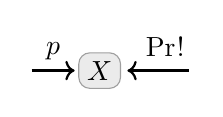
\begin{tikzpicture}[center base]
			\node[dpad0] (X) {$X$};
			\coordinate (A) at ($(X) + (-0.9,0)$);
			\draw[arr1] (A) -- node[above]{$p$}  (X);
			\draw[arr2, <-] (X) --  node[above,pos=0.6]{${\datadist\xsamp}!$} ++(1.2, 0);
				%\overset{\{\beta = \infty\}}
		\end{tikzpicture}
		}_\gamma + (1+\gamma) \H(\datadist\xsamp)
		\)
	% \item
	% \(\aar[\Bigg] {
	% 	\begin{tikzpicture}[center base]
	% 		\node[dpad0] (X) {$X$};
	% 		\coordinate (A) at ($(X) + (-1.2,0)$);
	% 		\draw[arr1] (A) -- node[above,pos=0.4]{$ \overset {\{\alpha = 1\}} p$}  (X);
	% %
	% 		\draw[arr2, <-] (X) --  node[above,pos=0.6]{$ \overset{\{\beta = \infty,\alpha=\gamma\}}{\datadist\xsamp}$} ++(1.5, 0);
	% 	\end{tikzpicture}
	% 	}\!\bigg._1 \)
\end{enumerate}
\end{prop}
\begin{proof}
	The equality of 1 and 2 is standard. The equality of 3 and 4 can be seen by the fact that in the limit of infinite confidence on $\datadist\xsamp$, the optimal distribution must also equal $\datadist\xsamp$, so the least inconsistency is attained at this value.
	Finally it remains to show that the first two and last two are equal:
	\begin{align*}
		\bbr{\,p\,}_\gamma(\datadist\xsamp) + (1+\gamma)\H(\datadist\xsamp)
		&=  \kldiv{\datadist\xsamp}{p} - \gamma \H(\datadist\xsamp)+ (1+\gamma)\H(\datadist\xsamp) \\
		&= \kldiv{\datadist\xsamp}{p} + \H(\datadist\xsamp) \\
		&= \Ex\nolimits_{\datadist\xsamp}\left[\log\frac{\datadist\xsamp}{p} +  \log\frac{1}{\datadist\xsamp}\right]
		= \Ex\nolimits_{\datadist\xsamp}\left[\log\frac{1}{p}\right],
	\end{align*}
	which is the cross entropy, as desired.
\end{proof}

\begin{remark}
Note that the entropy of the data distribution $\H(\datadist\xsamp)$ is constant in $p$, and so this additional term in (3, 4) as well as the the qualitative components of the PDGs, are irrelevant if we intend to optimize this objective by varying $p$.
\end{remark}

We argue that the PDGs in \cref{prop:many-equal-simple} are natural. Aside from the weights, this should be uncontroversial --- we've simply translated the entire problem into a set of probability distributions and included them into the PDG.
In the current setting, we argue that the weights are also the ones we would expect. The cross entropy measures the expected code length per sample, when a (possibly incorrect) distribution $p$ is used to design a code, in place of the true one $\datadist\xsamp$.
So implicitly, a modeler who chooses a cross-entropy objective believes that the data distribution is the ``true one'', and has much higher certainty in $\datadist\xsamp$ than in $p$. This justifies the `!'.
Other choices of $\beta$ are more natural in other contexts, and we will see later that they correspond to other losses. (For instance when $\beta_p = \beta_{\datadist\xsamp} = \frac12$, the result is the Bhattacharyya distance, rather than the cross entropy.)

% Furthermore, $p$ is the qualitative model we have in mind, and so we set $\alpha_p = 1$

We also get an analog of \Cref{prop:marginal-ll} in the partially observed case.
\begin{prop}
		\label{prop:pdg-loglikelihood}
	The average negative log likelihood $-\frac{1}{|\xsamp|}\sum_{x \in \xsamp} \log p(x)$ (i.e., the cross entropy) is the inconsistency of the PDG containing $p$ and the data distribution $\datadist\xsamp$.
	That is,
	\[
	\ell(p;\xsamp) =
	 \aar[\Bigg]{
	 % \Inc\left(
		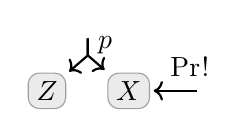
\begin{tikzpicture}[center base]
			\node[dpad0] (Z) {$Z$};
			\node[dpad0,right=.5 of Z] (X) {$X$};
			\coordinate (A) at ($ (X)!.5!(Z) + (0,0.7)$);
			\draw[arr1] (A) -- node[right]{$p$} ++(0,-0.25) -- (X);
			\draw[arr1] (A) -- ++(0,-0.25) -- (Z);
			%
			\draw[arr1, <-] (X) --  node[above,pos=0.8]{$\datadist\xsamp!$} ++(0.9, 0);
			% \draw[arr1, <-] (Z) -- node[above]{$\scriptstyle q$} ++(-0.9, 0);
		\end{tikzpicture}
		}%_{\!\!0}
		% \right)
		+ \H(\datadist\xsamp).
	\]
\end{prop}
\begin{proof}
	The same idea as in \cref{prop:marginal-ll}, but a little more complicated.

	\begin{align*}
	\aar*{
		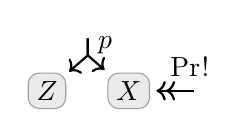
\begin{tikzpicture}[center base]
			\node[dpad0] (Z) {$Z$};
			\node[dpad0,right=.5 of Z] (X) {$X$};
			\coordinate (A) at ($ (X)!.5!(Z) + (0,0.7)$);
			\draw[arr1] (A) -- node[right]{$p$} ++(0,-0.25) -- (X);
			\draw[arr1] (A) -- ++(0,-0.25) -- (Z);
			\draw[arr2, <<-] (X) --  node[above,pos=0.8]{$\datadist\xsamp!$} ++(0.9, 0);
		\end{tikzpicture}}
			&= \inf_{\mu(Z \mid X)} \bbr*{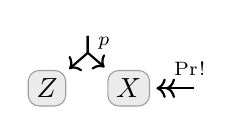
\begin{tikzpicture}[center base]
				\node[dpad0] (Z) {$Z$};
				\node[dpad0,right=.5 of Z] (X) {$X$};
				\coordinate (A) at ($ (X)!.5!(Z) + (0,0.7)$);
				\draw[arr1] (A) -- node[right]{$\scriptstyle p$} ++(0,-0.25) -- (X);
				\draw[arr1] (A) -- ++(0,-0.25) -- (Z);
				\draw[arr2, <<-] (X) --  node[above,pos=0.8]{$\scriptstyle \datadist\xsamp!$} ++(0.9, 0);
			\end{tikzpicture}}\Big(\datadist\xsamp(X) \mu(Z \mid X)\Big)  \\
			&= \inf_{\mu(Z \mid X)}\kldiv[\Big]{\datadist\xsamp(X) \mu(Z \mid X)}{p(X,Z)} \\
			&= \inf_{\mu(Z \mid X)}
				\Ex_{\substack{x \sim \datadist\xsamp \\ z \sim \mu}}
					\log \frac{\mu(z \mid x)\datadist\xsamp(x)}{p(x,z)} \\
			&= \frac{1}{|\xsamp|}\inf_{\mu(Z\mid X)}\sum_{x \in \xsamp}
				\Ex_{z \sim \mu(Z\mid x)} \log \frac{\mu(z \mid x) \datadist\xsamp(x) }{p(x,z)}\frac{p(x)}{p(x)} \\
			&= \frac{1}{|\xsamp|}\inf_{\mu(Z \mid X)}\sum_{x \in \xsamp}\Ex_{z \sim \mu} \left[ \log \frac{\mu(z)}{p(z \mid x)} + \log \frac{1}{p(x)} - \log \frac{1}{\datadist\xsamp(x)} \right] \\
			&= \frac{1}{|\xsamp|}\sum_{x \in \xsamp} \left[
				\inf_{\mu(Z)} \Big[\kldiv{\mu(Z)}{p(Z\mid x)}\Big] + \log \frac{1}{p(x)} \right] - \H(\datadist\xsamp) \\
			&= \frac{1}{|\xsamp|}\sum_{x \in \xsamp} \log \frac{1}{p(x)} - \H(\datadist\xsamp)
			= \frac{1}{|\xsamp|} \sum_{x \in \xsamp} I_p(x) - \H(\datadist\xsamp) \\
			\Big(\quad&= \kldiv{\datadist\xsamp}{p(X)} \quad \Big)
	\end{align*}
\end{proof}

We can also prove results of a similar flavor in the supervised case.
\begin{prop}
	Consider a probabilistic model $f(y\mid x)$ for supervised regression or classification. The inconsistency of the PDG containing $p(y \mid x)$ and the emperical distribution of samples $\xysamp$ is equal to the negative log-liklihood (cross-entropy) loss, up to a constant independent of $f$ (the entropy of the data). That is,
	\[ \aar*{
		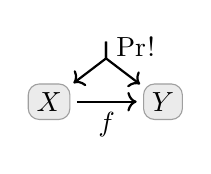
\begin{tikzpicture}[center base]
			\node[dpad0] (Y) {$Y$};
			\node[dpad0,left=.9 of Y] (X) {$X$};
			\coordinate (A) at ($ (X)!.5!(Y) + (0,0.8)$);
			\draw[arr1] (A) -- node[right]{$\datadist\xysamp!$} ++(0,-0.25) -- (X);
			\draw[arr1] (A) -- ++(0,-0.25) -- (Y);
			\draw[arr2, ->] (X) --  node[below,pos=0.5]{$f$} (Y);
		\end{tikzpicture}} = \frac1{|\xysamp|}\sum_{(x,y) \in \xysamp} \log \frac1{f(y \mid x)} \quad + \H(\datadist\xysamp)
	\]
\end{prop}
\begin{proof}
	This is immediate, since $\datadist\xysamp$ has high confidence, and $f$ is the only other edge.
\end{proof}

\subsection{Simple Performance Metrics as Inconsistencies}

There are also simpler scoring metrics used to evaluate the performance of systems on datasets, such as the accuracy of a  classifier, or the mean-squared error of a regressor?

\begin{prop}[classification accuracy as inconsistency]
	\label{prop:accuracy}
	If $h: X \to Y$ is a classifier for an input space $X$ and label space $Y$, and $f: X \to Y$ generates the correct labels, then the inconsistency of believing $f$ and $h$ (with any conficences), and that inputs are distributed according to $D(X)$ (with confidence $\beta$), equals the log accuracy of $h$ on $D$, times $\beta$. That is,
	\begin{equation}\label{eq:accuracy-pdg}
		\aar*{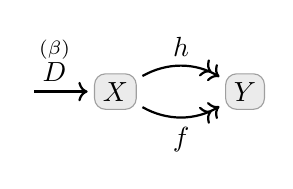
\begin{tikzpicture}[center base]
				\node[dpad0] (Y) {$Y$};
				\node[dpad0,left=1.1 of Y] (X) {$X$};
				%
				\draw[arr2, ->>] (X) to[bend left] node[pos=0.5, above]{$h$} (Y);
				\draw[arr2, ->>] (X) to[bend right] node[pos=0.5, below]{$f$} (Y);
				\draw[arr2, <-] (X) to node[pos=0.6, above]{$\overset{(\beta)}D$} +(-1.1, 0);
			\end{tikzpicture}}
		=  \beta\,\log \Big( \mathrm{accuracy}_{D} (h) \Big).
	\end{equation}
\end{prop}
We often think of accuracy as a property of a hypothesis $h$ with respect to the true labeling function $f$, but the correspondence of \Cref{prop:accuracy} highlights graphically both its symmmetry ($f$ and $h$ play exactly the same role), and the particularly strong dependence on the distribution of inputs.
In fact, the the expression for the inconsistency of the PDG in \eqref{eq:accuracy-pdg} does not depend on the confidences in $h$ or $f$, so

%Confusion matrix costs
\begin{prop}
	\[
	\]
\end{prop}


When $Y$ is a continuous variable rather than a discrete one, the estimator is referred to as a regressor, rather than a classifier, and often we use mean squared error, rather than

\begin{prop}[Mean squared error as inconsistency]
	\begin{align*}
		\aar*{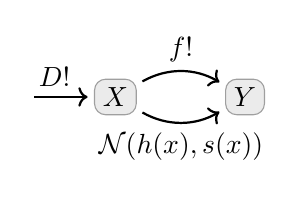
\begin{tikzpicture}[center base]
			\node[dpad0] (Y) {$Y$};
			\node[dpad0,left=1.1 of Y] (X) {$X$};
			%
			\draw[arr2, ->] (X) to[bend left]
				node[pos=0.5, above] {$f!$} (Y);
			\draw[arr2, ->] (X) to[bend right]
				node[pos=0.5, below]{$\mathcal N(h(x), s(x))$} (Y);
			\draw[arr2, <-] (X) to node[pos=0.6, above]{$D!$} +(-1.1, 0);
		\end{tikzpicture}}
		&=
		\aar*{
		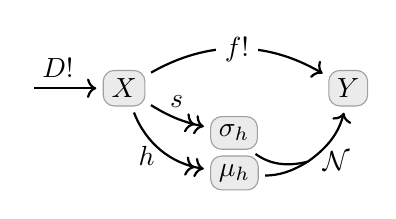
\begin{tikzpicture}[scale=1.1,center base]
			\node[dpad0] (Y) {$Y$};
			\node[dpad0,left=2.3 of Y] (X) {$X$};
			% \node[dpad0,above left=0.5 and 1.1 of Y] (mf) {$\mu_f$};
			\node[dpad0,below right=0.6 and 0.8 of X] (mh) {$\mu_h$};
			% \node[dpad0,above left=0.2 and 0.8 of Y] (sf) {$\sigma_f$};
			\node[dpad0,below right=0.1 and 0.8 of X] (sh) {$\sigma_h$};
			%
			% \draw[arr2, ->>] (X) to[bend left]
			% 	node[pos=0.5, above] {$f$} (mf);
			% 	\draw[arr2, ->>] (X) to[bend left]
			% 		node[pos=0.5, above] {$t$} (sf);
			\draw[arr2, ->>] (X) to[bend right=30]
				node[pos=0.6, left] {$h$\,} (mh);
				\draw[arr2, ->>] (X) to[bend right=10]
					node[pos=0.5, above] {$s$} (sh);
			%
			\draw[arr2, <-] (X) to node[pos=0.6, above]{$D!$} +(-1.1, 0);
			\draw[arr2, ->] (X) to[bend left]
			 	node[pos=0.5, fill=white]{$f!$} (Y);
			\coordinate (C1) at ($(mh)!.5!(sh) + (0.85,-0.1)$);
			% \coordinate (C2) at ($ (X)!.5!(Y) + (0,0.8)$);
			\draw[arr2, ->] (mh) to[bend right=15] (C1) to[bend right=20]
			 	node[pos=0.25, below right, inner sep=0] {$\mathcal N$} (Y);
			\draw[arr2, -,shorten >=0pt] (sh) to[bend right=25] (C1);
			% \draw (current bounding box.north east) rectangle (current bounding box.south west);
		\end{tikzpicture}}\\
		 &= \Ex\nolimits_D \left[
		  	2 \log f(Y \mid X) + \frac\beta2\frac{(Y-h(X))^2}{s(X)^2}
				+ \log 2\pi s(X)^2 \right]
	\end{align*}
\end{prop}
The first equation

\begin{defn}[power mean]
	The weighted power mean $\mathrm M^w_p(r_1, \ldots, r_n)$ of the real numbers $r_1, \lodts, r_n$ with respect to weights $w = w_1, \ldots, w_n$ satisfying $\sum_iw_i = 1$, is given by
	\[ \mathrm M^w_p(r_1, \ldots, r_n) := \left(\sum_i w_i (r_i)^p \right)^{\frac1p}\]
\end{defn}

\begin{prop}
	\[
		\aar*{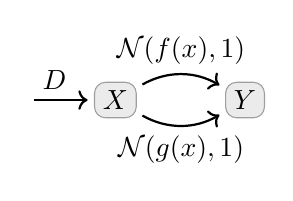
\begin{tikzpicture}[center base]
			\node[dpad0] (Y) {$Y$};
			\node[dpad0,left=1.1 of Y] (X) {$X$};
			%
			\draw[arr2, ->] (X) to[bend left]
				node[pos=0.5, above] {$\mathcal N(f(x), 1)$} (Y);
			\draw[arr2, ->] (X) to[bend right] node[pos=0.5, below]{$\mathcal N(g(x), 1)$} (Y);
			\draw[arr2, <-] (X) to node[pos=0.6, above]{$D$} +(-1.1, 0);
		\end{tikzpicture}}
		 = \Ex\nolimits_D \left[ \left( \frac{f(X) - h(X)}
		 	{\mathrm M_2^{\hat\beta}\{\sigma_1,\sigma_2\}} \right)^2 + (\beta_1 + \beta_2) \log
		 	\frac
				{\mathrm M_2^{\hat\beta}(\sigma_1,\sigma_2)}
				{\mathrm M_0^{\hat\beta}(\sigma_1,\sigma_2)}
		 \right]
	\]
	where $\hat\beta = (\frac{\beta_2}{\beta_1+\beta_2}, \frac{\beta_1}{\beta_1+\beta_2})$
\end{prop}

\begin{coro}[Mean Square Error]
	\[
		\aar*{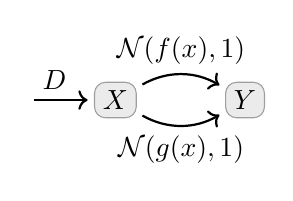
\begin{tikzpicture}[center base]
			\node[dpad0] (Y) {$Y$};
			\node[dpad0,left=1.1 of Y] (X) {$X$};
			%
			\draw[arr2, ->] (X) to[bend left]
				node[pos=0.5, above] {$\mathcal N(f(x), 1)$} (Y);
			\draw[arr2, ->] (X) to[bend right] node[pos=0.5, below]{$\mathcal N(g(x), 1)$} (Y);
			\draw[arr2, <-] (X) to node[pos=0.6, above]{$D$} +(-1.1, 0);
		\end{tikzpicture}}
		 = \Ex\nolimits_D \Big( f(X) - h(X) \Big)^2
		 =: \mathrm{MSE}( f, h )
	\]
\end{coro}

Although the results in this section are not particularly useful on their own, they do hint at a surprisingly strong tie between the standard metrics used to train probabilistic models, and the inconsistency of a corresponding PDG ---
we have seen that (marginal) log likelihood, cross entropy, and log accuracy all arise naturally as inconsistencies of the appropriate PDGs.


%%%%%%%%%%%%%%%%%%%%%%%%%%%%%%%%%%%%%%%%%%%%%%%%%%%%%%%%%%%%%%%%%%%%%%%%%%
\section{Statistical Distances as Inconsistencies}
Suppose you are concerned with only a single variable $X$. One friend has told you that it is distributed according to the probabiltiy distribution $p(X)$; another has told you that it follows $q(X)$. You adopt both beliefs. If $p \ne q$, your mental state will be inconsistent, and moreso, the more $p$ and $q$ differ.
Thus, we can think of the inconsistency of a PDG containing only a single varible $X$ and two distributions $p(X)$ and $q(X)$ over it, as a measure of divergence.

Recall that a PDG also allows us to specify the confidences $\beta_p$ and $\beta_q$ of each edge, and as we vary them, the resulting measure of inconsistency reduces to a surprisingly large classs of statistical distances.

\begin{lemma}
    \[
        \aar[\bigg]{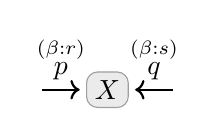
\begin{tikzpicture}[center base]
            \node[dpad0] (X) {$X$};
            \draw[arr2, <-] (X) -- node[above]
                {$\overset{(\beta : r)}p$}  ++(-0.9,0);
            \draw[arr2, <-] (X) --  node[above,pos=0.5]
                {$\overset{(\beta : s)}q$} ++(0.9, 0);
        \end{tikzpicture}}
        % = \thickD^{\mathrm{PDG}}_{(r,s)}(p, q)
        = - (r+s) \log  \sum_x \left(p(x)^{r}\vphantom{\Big|} q(x)^{s}\right)^{\frac{1}{r+s}}
        % = - (r+s) \log \sum_x \! \sqrt[\leftroot{0}\uproot{2}r+s]{\vphantom{\big|}p(x)^{r} q(x)^{s}}
    % \qquad\text{where}\qquad \xi:= \beta_p+\beta_q
    \]
\end{lemma}


\begin{prop}[KL divergence]
\[
    \kldiv pq =
    \aar*{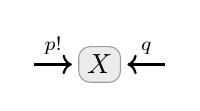
\begin{tikzpicture}[center base]
        \node[dpad0] (X) {$X$};
        \draw[arr2, <-] (X) -- node[above]
            {$\scriptstyle p !$}  ++(-0.9,0);
        \draw[arr2, <-] (X) --  node[above,pos=0.5]
            {$\scriptstyle q$} ++(0.9, 0);
    \end{tikzpicture}}
\]
\end{prop}
This result gives us an intuitive interpretation of the asymmetry of the KL divergence, the counter-intuitive naming of itsarguments, and a prescription about when it makes most sense to use it.
$\kldiv p q$ is the inconsistency of a mental state when absolutely certain of $p$ (and not willing to budge on it), which is why it reflects the amount of information required to change $p$ into $q$, and why we call it the divergence from $q$ to $p$.


\begin{prop}[Reny\'i Divergences]
    \[ \thickD^{\mathrm{PDG}}_{r, s}(p, q) =
        s \cdot \thickD_{\frac{r}{r+s}}\infdivx{p}{q}
    \qquad \text{and} \qquad
        \thickD_{\alpha}\infdivx{p}{q}
        = \thickD^{\mathrm{PDG}}_{\left(\frac{\alpha}{1-\alpha}, 1\right)}(p, q)
    \]
\end{prop}



\begin{prop}[Chernoff Divergences]
\[
	\aar[\bigg]{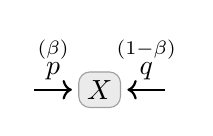
\begin{tikzpicture}[center base]
		\node[dpad0] (X) {$X$};
		\draw[arr2, <-] (X) -- node[above]
			{$\overset{(\beta)}p$}  ++(-0.9,0);
		\draw[arr2, <-] (X) --  node[above,pos=0.5]
			{$\overset{(1-\beta)}q$} ++(0.9, 0);
	\end{tikzpicture}}
	% = \thickD^{\mathrm{PDG}}_{(r,s)}(p, q)
	= - (r+s) \log  \sum_x \left(p(x)^{r}\vphantom{\Big|} q(x)^{s}\right)^{\frac{1}{r+s}}
	% = - (r+s) \log \sum_x \! \sqrt[\leftroot{0}\uproot{2}r+s]{\vphantom{\big|}p(x)^{r} q(x)^{s}}
% \qquad\text{where}\qquad \xi:= \beta_p+\beta_q
\]
\end{prop}




\section{Varitaional Objectives and Bounds}
\label{sec:theory}


% \todo add the equivalence results between PDGs and VAEs



The fact that the incompatibility of $\dg M$ with a \emph{specific} joint distribution $\mu$ is an upper bound on the inconsistency (i.e., the score of the \emph{best} such joint distribution) does not seem terribly deep, even if it does end up yielding an inference procedure for PDGs of a variational flavor (that is, choose a tractable parametric family of distributions $\mu$, and use it to optimize based on inconsistency, and thereby draw inferences).

Perhaps surprisingly, the converse is also true: variational inference is captured by the internal workings of a PDG.  Moreover, PDGs give a concise graphical language for this kind of reasoning, which can be notoriously difficult to track symbolically.

We begin with `evidence lower bound', or the ELBO, which is a common objective for training latent variable models.
Suppose we have a joint distribution $p(X,Z)$, but only have access to observations $X$. Evaluating $p(X)$ requires marginalizing over $Z$, and could be intractable if $Z$ is complex. One workaround is to instead suppose that $Z$ is distributed according to a simple parametric family $q_\theta(Z)$.
In this case, the ELBO \eqref{eq:elbo} is easier to compute, and seems in practice to work for training models in practice.
\begin{equation}
	\mathrm{ELBO}_{p,q}(x) := \Ex_{z \sim q} \log \frac{p(x,z)}{q(z)} \label{eq:elbo}
\end{equation}

% We will now see that this tie extends to latent variable models in a nice way.
It turns out that the ELBO also arises naturally as a PDG inconsistency.

\begin{prop}\label{prop:pdg-elbo-x}%[Capturing the ELBO]
		% \label{prop:pdg-elbo-x}
	% If $p(X,Z)$ is a joint probabilistic model of observed variables $X$ and hidden variables $Z$, and $q(Z)$ is any distribution
	% That is,
	The negative ELBO is the inconsistency of the PDG containing $p,q$, and $x$, with very high confidence in $q$.
	That is,
	\[
	-\mathrm{ELBO}_{p,q}(x) =
		% \lim_{t \to \infty}
	 \aar[\Bigg]{
% 	  \Inc\left(
		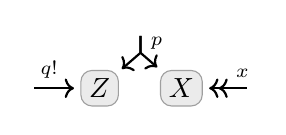
\begin{tikzpicture}[center base]
			\node[dpad0] (Z) {$Z$};
			\node[dpad0,right=.5 of Z] (X) {$X$};
			\coordinate (A) at ($ (X)!.5!(Z) + (0,0.7)$);
			\draw[arr1] (A) -- node[right]{$\scriptstyle p$} ++(0,-0.25) -- (X);
			\draw[arr1] (A) -- ++(0,-0.25) -- (Z);
%
			\draw[arr2, <<-] (X) --  node[above,pos=0.8]{$\scriptstyle x$} ++(0.9, 0);
			\draw[arr2, <-] (Z) -- node[above,pos=0.6]{$\scriptstyle q!$} ++(-0.9, 0);%
			%\scriptstyle q^{\{\beta =\infty\}}
			% \ar[r,"p"] \& Z \ar[r,"p", bend left] \& X \ar[l,"q", bend left] \& \ar[l, two heads, "x"']
		\end{tikzpicture}
		}%_{\!\!0}
% 		\right)
		.
	\]
\end{prop}
\begin{proof}
	Every distribution that does marginalize to $q(Z)$ or places any mass on $x' \ne x$ will have infinite score. Thus the only distribution that could have a finite score is $\mu(X,Z)$. Thus,

	\begin{align*}
	\aar[\Bigg]{
% 	  \Inc\left(
	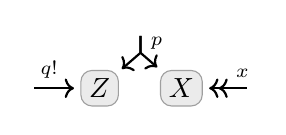
\begin{tikzpicture}[center base]
		\node[dpad0] (Z) {$Z$};
		\node[dpad0,right=.5 of Z] (X) {$X$};
		\coordinate (A) at ($ (X)!.5!(Z) + (0,0.7)$);
		\draw[arr1] (A) -- node[right]{$\scriptstyle p$} ++(0,-0.25) -- (X);
		\draw[arr1] (A) -- ++(0,-0.25) -- (Z);
%
		\draw[arr2, <<-] (X) --  node[above,pos=0.8]{$\scriptstyle x$} ++(0.9, 0);
		\draw[arr2, <-] (Z) -- node[above,pos=0.6]{$\scriptstyle q!$} ++(-0.9, 0);%
		%\scriptstyle q^{\{\beta =\infty\}}
		% \ar[r,"p"] \& Z \ar[r,"p", bend left] \& X \ar[l,"q", bend left] \& \ar[l, two heads, "x"']
	\end{tikzpicture}
	}
	 &= \inf_\mu \bbr*{
% 	  \Inc\left(
		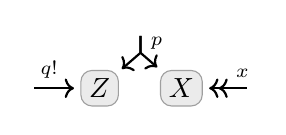
\begin{tikzpicture}[center base]
			\node[dpad0] (Z) {$Z$};
			\node[dpad0,right=.5 of Z] (X) {$X$};
			\coordinate (A) at ($ (X)!.5!(Z) + (0,0.7)$);
			\draw[arr1] (A) -- node[right]{$\scriptstyle p$} ++(0,-0.25) -- (X);
			\draw[arr1] (A) -- ++(0,-0.25) -- (Z);
%
			\draw[arr2, <<-] (X) --  node[above,pos=0.8]{$\scriptstyle x$} ++(0.9, 0);
			\draw[arr2, <-] (Z) -- node[above,pos=0.6]{$\scriptstyle q!$} ++(-0.9, 0);%
			%\scriptstyle q^{\{\beta =\infty\}}
			% \ar[r,"p"] \& Z \ar[r,"p", bend left] \& X \ar[l,"q", bend left] \& \ar[l, two heads, "x"']
		\end{tikzpicture}
		}( \mu ) \\
	  &= \bbr*{
 % 	  \Inc\left(
 		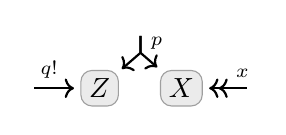
\begin{tikzpicture}[center base]
 			\node[dpad0] (Z) {$Z$};
 			\node[dpad0,right=.5 of Z] (X) {$X$};
 			\coordinate (A) at ($ (X)!.5!(Z) + (0,0.7)$);
 			\draw[arr1] (A) -- node[right]{$\scriptstyle p$} ++(0,-0.25) -- (X);
 			\draw[arr1] (A) -- ++(0,-0.25) -- (Z);
 %
 			\draw[arr2, <<-] (X) --  node[above,pos=0.8]{$\scriptstyle x$} ++(0.9, 0);
 			\draw[arr2, <-] (Z) -- node[above,pos=0.6]{$\scriptstyle q!$} ++(-0.9, 0);%
 			%\scriptstyle q^{\{\beta =\infty\}}
 			% \ar[r,"p"] \& Z \ar[r,"p", bend left] \& X \ar[l,"q", bend left] \& \ar[l, two heads, "x"']
 		\end{tikzpicture}
 		}( \delta_x(X) q(Z) ) \\
	 &= \Ex_{\substack{x' \sim \delta_x \\ z \sim q}} \log \frac{\delta_x(x')q(z)} {p(x',z)}
	 = - \Ex_{z \sim q} \frac{p(x,z)}{q(z)} = - \mathrm{ELBO}_{p,q}(x).
	\end{align*}
\end{proof}


%
% The proof of \cref{prop:pdg-elbo-x} %, lke that of \cref{prop:pdg-Ix},
%  hinges critically on the fact that we force a single sample $x$; its PDG does not capture the whole context $\xsamp$.
% Nevertheless, we get an analogous result when we replace the sample $x$ with the entire data distribution $\datadist\xsamp$, which differs only in that the expression is offset by the entropy of the data distribution.
%
%
% \begin{prop}\label{prop:pdg-elbo-X}
% 	Consider a model $p(X,Z)$, auxiliary distribution $q(Z)$, and samples $\xsamp = \{x^{(i)}\}$ defining a data distribution $\datadist\xsamp$.
% 	The following are equal:
% 	\begin{enumerate}[label=(\arabic*)]
% 		\item $- \Ex_{\datadist\xsamp} \mathrm{ELBO}_{p,q}(X)$
% 		\item $\displaystyle\bbr{\,p\,}(q \otimes \datadist\xsamp) + \H(\datadist\xsamp)$
% 		\item \(\displaystyle%\lim_{\beta_q, \beta_{\datadist\xsamp} \to \infty}
% 			% \lim_{t \to \infty}
% 		  \aar[\Bigg]{
% 		  \begin{tikzpicture}[center base]
% 	  		\node[dpad0] (Z) {$Z$};
% 	  		\node[dpad0,right=.5 of Z] (X) {$X$};
% 	  		\coordinate (A) at ($ (X)!.5!(Z) + (0,0.7)$);
% 	  		\draw[arr1] (A) -- node[right]{$\scriptstyle p$} ++(0,-0.25) -- (X);
% 	  		\draw[arr1] (A) -- ++(0,-0.25) -- (Z);
% 	  %
% 	  		\draw[arr1, <-] (X) --  node[above,pos=0.2,anchor=south west]{$\scriptstyle {\datadist\xsamp}!$} ++(0.9, 0);
% 	  			% ^{\{\beta=\beta_0\}}
% 	  		\draw[arr1, <-] (Z) -- node[above]{$\scriptstyle q! $} ++(-0.9, 0);
% 	  	\end{tikzpicture} }_1 + \H(\datadist\xsamp)\)
% 	\end{enumerate}
%
% \end{prop}
% \begin{proof}
%
% \end{proof}



The use of the ELBO as an objective is often justified by the fact that it lower-bounds the objective that you ``really wanted'': the cross entropy.
This is often proved by jensen's inequality, or alternatively, but appeal to the non-negativity of relative entropy \cite{elboproofs}.
We now give a very simple, different-looking diagrammatic proof of this second approach, by appealing to the intuitive fact that adding believing more things cannot make you less inconsistent, as captured by \cref{lemma!}.

\[
\log \frac{1}{p(x)} =
    % \lim_{t \to \infty}
	 \aar[\Bigg]{
% 	  \Inc\left(
		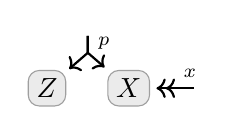
\begin{tikzpicture}[center base]
			\node[dpad0] (Z) {$Z$};
			\node[dpad0,right=.5 of Z] (X) {$X$};
			\coordinate (A) at ($ (X)!.5!(Z) + (0,0.7)$);
			\draw[arr1] (A) -- node[right]{$\scriptstyle p$} ++(0,-0.25) -- (X);
			\draw[arr1] (A) -- ++(0,-0.25) -- (Z);
%
			\draw[arr2, <<-] (X) --  node[above,pos=0.8]{$\scriptstyle x$} ++(0.9, 0);
% 			\draw[arr2, <-] (Z) -- node[above,pos=0.6]{$\scriptstyle q^{\{\beta =\infty\}}$} ++(-0.9, 0);%
			% \ar[r,"p"] \& Z \ar[r,"p", bend left] \& X \ar[l,"q", bend left] \& \ar[l, two heads, "x"']
		\end{tikzpicture}
		}%_{\!\!0}
% 		\right)
	\le
    % \lim_{t \to \infty}
	 \aar[\Bigg]{
% 	  \Inc\left(
		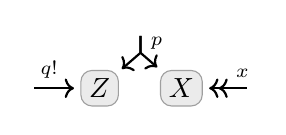
\begin{tikzpicture}[center base]
			\node[dpad0] (Z) {$Z$};
			\node[dpad0,right=.5 of Z] (X) {$X$};
			\coordinate (A) at ($ (X)!.5!(Z) + (0,0.7)$);
			\draw[arr1] (A) -- node[right]{$\scriptstyle p$} ++(0,-0.25) -- (X);
			\draw[arr1] (A) -- ++(0,-0.25) -- (Z);
%
			\draw[arr2, <<-] (X) --  node[above,pos=0.8]{$\scriptstyle x$} ++(0.9, 0);
			\draw[arr2, <-] (Z) -- node[above,pos=0.6]{$\scriptstyle q!$} ++(-0.9, 0);%
			% \ar[r,"p"] \& Z \ar[r,"p", bend left] \& X \ar[l,"q", bend left] \& \ar[l, two heads, "x"']
		\end{tikzpicture}
		}%_{\!\!0}
% 		\right)
    = -\mathrm{ELBO}_{p,q}(x),
\]

The first and last equalities are \Cref{prop:marginal-ll,prop:pdg-elbo-x}, and
the inequality is due to \Cref{lemma!}.
Compared to the standard proofs, the motivation can be seen quite easily: the second PDG has more edges. We also have analog analog holds for the entire dataset at once, which is more easily formulated with a slightly different variational form in the next section.

% \begin{align*}
% \ell(p;\xsamp) &=
% 	 \aar[\Bigg]{
% 	 % \Inc\left(
% 		\begin{tikzpicture}[center base]
% 			\node[dpad0] (Z) {$Z$};
% 			\node[dpad0,right=.5 of Z] (X) {$X$};
% 			\coordinate (A) at ($ (X)!.5!(Z) + (0,0.7)$);
% 			\draw[arr1] (A) -- node[right]{$\scriptstyle p$} ++(0,-0.25) -- (X);
% 			\draw[arr1] (A) -- ++(0,-0.25) -- (Z);
% %
% 			\draw[arr1, <<-] (X) --  node[above,pos=0.8]{$\scriptstyle \datadist\xsamp$} ++(0.9, 0);
% 			% \draw[arr1, <-] (Z) -- node[above]{$\scriptstyle q$} ++(-0.9, 0);
% 		\end{tikzpicture}
% 		}%_{\!\!0}
% 		% \right)
% 		 + \H(\datadist\xsamp) \\
% 		&\le
% 			\lim_{t \to \infty}
% 		  \aar[\Bigg]{
% 		  \begin{tikzpicture}[center base]
% 	  		\node[dpad0] (Z) {$Z$};
% 	  		\node[dpad0,right=.5 of Z] (X) {$X$};
% 	  		\coordinate (A) at ($ (X)!.5!(Z) + (0,0.7)$);
% 	  		\draw[arr1] (A) -- node[right]{$\scriptstyle p$} ++(0,-0.25) -- (X);
% 	  		\draw[arr1] (A) -- ++(0,-0.25) -- (Z);
% 	  %
% 	  		\draw[arr1, <-] (X) --  node[above,pos=0.2,anchor=south west]{$ {\datadist\xsamp}^{\{\beta= t\}}$} ++(0.9, 0);
% 	  			% ^{\{\beta=\beta_0\}}
% 	  		\draw[arr1, <-] (Z) -- node[above]{$q^{\{\beta= t\}} $} ++(-0.9, 0);
% 	  	\end{tikzpicture} } + \H(\datadist\xsamp) = - \Ex_{\datadist\xsamp} \mathrm{ELBO}_{p,q}(X),
% \end{align*}
% which holds for the same reason.


\subsection{Variational Auto-Encoders and PDGs}

An autoencoder is a probabilistic model intended to compress a variable $X$ (e.g., an image) to a compact latent representation $Z$ (a compact vector), and is specified by two conditional distributions:
an encoder $e(Z \mid X)$, and a decoder $d(X \mid Z)$.
Of course, not all pairs of cpds fill this role equally well.
Perhaps most importantly, we would to have low \emph{reconstruction error} \eqref{eq:rec}---when we decode an encoded image, we would like it to be reasonably similar to the original.

\begin{equation}
 \mathrm{Rec}(x) = \Ex_{z \sim e \mid x} \underbrace{\mathrm I_{d\mid z}[x]}_{\substack{\text{Additional bits to}\\\text{specify $x$ from $d|z$}}}
	= \sum_z e(z \mid x) \log \frac1{d(x \mid z)}\label{eq:rec}
\end{equation}

% Note the similarity to the cross entropy objective from before, except in place of our

There are other desiderata as well. It would be nice if the distribution on $Z$ had a simple form---perhaps factoring into independent features, which we might use to describe $X$. To deal with this, we can introduce a new distribution $p(Z)$

In this setting, $e$ is our variational approximation to the latent variables, and differs from $q$ in the previous section, in that it can now depend on $X$. The evidence lower bound now becomes
\begin{align*}
	\mathrm{ELBO}_{p,e,d}(x) &= \Ex_{z \sim e|x} \left[\log \frac{p(z) d(x\mid z)}{e(z\mid x)} \right] \\
		&= \Ex_{z \sim e|x}\left[ \log \frac{p(z)}{e(z\mid x)}  \right] - \Ex_{z \sim e|x} \left[\log \frac1{d(x\mid z)} \right] \\
		&= \kldiv{e(Z|x)}{p} - \mathrm{Rec}(x)
\end{align*}

In this setting, we get a result analogous to Proposition~\ref{prop:pdg-elbo-x}.

\begin{prop}\label{prop:pdg-elbo-vae}
	The conditional ELBO used as a VaE objective is the inconsistency of the PDG containing the encoder $e$, decoder $d$ prior $p$, and a sample $x$.
	That is,
	\[
	-\mathrm{ELBO}_{p,e,d}(x) =
	 \aar*{
		% \begin{tikzcd}[AmpRep,row sep=1em,column sep=1.5em]
		% 	\ar[r,"p"] \& Z \ar[r,"d", bend left] \& X \ar[l,"e!", bend left] \& \ar[l, two heads, "x"']
		% \end{tikzcd}
		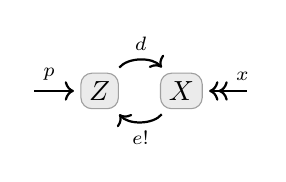
\begin{tikzpicture}[center base]
			\node[dpad0] (Z) {$Z$};
			\node[dpad0,right=.5 of Z] (X) {$X$};
			\draw[arr2, ->] (X) to[bend left=50]
				node[below]{$\scriptstyle e!$} (Z);
			\draw[arr2, ->] (Z) to[bend left=50]
				node[above]{$\scriptstyle d$} (X);
			\draw[arr2, <<-] (X) --
			  	node[above,pos=0.8]{$\scriptstyle x$}
			 	++(0.9, 0);
			\draw[arr2, <-] (Z) --
				node[above,pos=0.6]{$\scriptstyle p$}
				++(-0.9, 0);%
		\end{tikzpicture}}
	\]
\end{prop}
\begin{prop}\label{prop:pdg-elbo-vae-whole}
	The following analog of \cref{prop:pdg-elbo-vae} for a whole dataset $\xsamp$ holds:
	\[
	-\Ex_{\datadist\xsamp}\mathrm{ELBO}_{p,e,d}(X) =
	 \aar*{
		% \begin{tikzcd}[AmpRep,row sep=1em,column sep=1.5em]
		% 	\ar[r,"p"] \& Z \ar[r,"d", bend left] \& X \ar[l,"e!", bend left] \& \ar[l, two heads, "x"']
		% \end{tikzcd}
		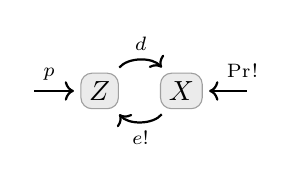
\begin{tikzpicture}[center base]
			\node[dpad0] (Z) {$Z$};
			\node[dpad0,right=.5 of Z] (X) {$X$};
			\draw[arr2, ->] (X) to[bend left=50]
				node[below]{$\scriptstyle e!$} (Z);
			\draw[arr2, ->] (Z) to[bend left=50]
				node[above]{$\scriptstyle d$} (X);
			\draw[arr2, <-] (X) --
				node[above,pos=0.8]{$\scriptstyle \datadist\xsamp!$}
				++(0.9, 0);
			\draw[arr2, <-] (Z) --
				node[above,pos=0.6]{$\scriptstyle p$}
				++(-0.9, 0);%
		\end{tikzpicture}} + \H(\datadist\xsamp). \]
\end{prop}
\begin{proof}
	This proofs of these propositions are simple. The optimal distribution must be $\delta_x(X) e(Z \mid X)$  or  $\datadist\xsamp(X) e(Z \mid X)$ (any other distribution gets infinite score). At the same time, $d$ and $p$ define a joint distribution, so the inconsistency in question becomes
	\[
		\kldiv[\Big]{\delta_x(X) e(Z \mid X)}{p(Z)d(X\mid Z)}
			 = \Ex_{z \sim e \mid x} \left[ \log \frac{p(z)d(x\mid z)}{e(z \mid x)} \right] = \mathrm{ELBO}_{p,e,d}(x)
	\]
	in the first, case, and
	\[ \kldiv[\Big]{\datadist\xsamp(X) e(Z \mid X)}{p(Z)d(X\mid Z)}
		 = \frac{1}{|\xsamp|}\sum_{x \in \xsamp} \Ex_{z \sim e \mid x} \left[ \log \frac{p(z)d(x\mid z)}{e(z \mid x)} + \log \frac{1}{\datadist\xsamp(x)} \right] = \mathrm{ELBO}_{p,e,d}(x) - \H(\datadist\xsamp)
	\]
	in the second.
\end{proof}

\subsubsection{Alternate Proofs of Variational Bounds}
\Cref{prop:pdg-elbo-vae,prop:pdg-elbo-vae-whole} can be used to derive the variational lower bound. Once again, the addition of the edge $e$ cannot decrease the inconsistency (\cref{lemma!}), but it makes it easier to identify and sample from the best-scoring distributions.
This result in the following simple visual proof:
\[
	- \log \Pr(x) =
	\aar*{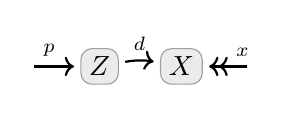
\begin{tikzpicture}[center base]
	   \node[dpad0] (Z) {$Z$};
	   \node[dpad0,right=.5 of Z] (X) {$X$};
	   \draw[arr2, ->] (Z) to[bend left=10]
		   node[above]{$\scriptstyle d$} (X);
	   \draw[arr2, <<-] (X) --
		   node[above,pos=0.8]{$\scriptstyle x$}
		   ++(0.9, 0);
	   \draw[arr2, <-] (Z) --
		   node[above,pos=0.6]{$\scriptstyle p$}
		   ++(-0.9, 0);%
	\end{tikzpicture}}
 	\le
 	\aar*{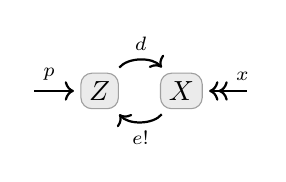
\begin{tikzpicture}[center base]
		\node[dpad0] (Z) {$Z$};
		\node[dpad0,right=.5 of Z] (X) {$X$};
		\draw[arr2, ->] (X) to[bend left=50]
			node[below]{$\scriptstyle e!$} (Z);
		\draw[arr2, ->] (Z) to[bend left=50]
			node[above]{$\scriptstyle d$} (X);
		\draw[arr2, <<-] (X) --
			node[above,pos=0.8]{$\scriptstyle x$}
			++(0.9, 0);
		\draw[arr2, <-] (Z) --
			node[above,pos=0.6]{$\scriptstyle p$}
			++(-0.9, 0);%
	\end{tikzpicture}} = -\mathrm{ELBO}_{p,e,d}(x).
\]
Here $\Pr(X)$ is the marginal of $p(Z)d(X \mid Z)$ on $X$.
\Cref{prop:pdg-elbo-vae-whole} lets us do the same thing for all datapoints at once, with only a single application of the inequality:

\[
	- \frac1{|\xsamp|}\sum_{x \in \datadist\xsamp} \log \Pr(x) =
	\aar*{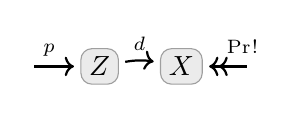
\begin{tikzpicture}[center base]
	   \node[dpad0] (Z) {$Z$};
	   \node[dpad0,right=.5 of Z] (X) {$X$};
	   \draw[arr2, ->] (Z) to[bend left=10]
		   node[above]{$\scriptstyle d$} (X);
	   \draw[arr2, <<-] (X) --
		   node[above,pos=0.8]{$\scriptstyle \datadist\xsamp!$}
		   ++(0.9, 0);
	   \draw[arr2, <-] (Z) --
		   node[above,pos=0.6]{$\scriptstyle p$}
		   ++(-0.9, 0);%
	\end{tikzpicture}}
 	\le
 	\aar*{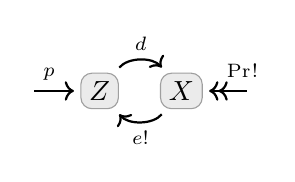
\begin{tikzpicture}[center base]
		\node[dpad0] (Z) {$Z$};
		\node[dpad0,right=.5 of Z] (X) {$X$};
		\draw[arr2, ->] (X) to[bend left=50]
			node[below]{$\scriptstyle e!$} (Z);
		\draw[arr2, ->] (Z) to[bend left=50]
			node[above]{$\scriptstyle d$} (X);
		\draw[arr2, <<-] (X) --
			node[above,pos=0.8]{$\scriptstyle \datadist\xsamp!$}
			++(0.9, 0);
		\draw[arr2, <-] (Z) --
			node[above,pos=0.6]{$\scriptstyle p$}
			++(-0.9, 0);%
	\end{tikzpicture}} = -\Ex_{\datadist\xsamp}\mathrm{ELBO}_{p,e,d}(X)
\]
\subsection{\texorpdfstring{$\beta$}{beta}-VaE Objective}

The ELBO is not the only objective to train VaEs. For instance, Higgins et. al. \cite{higgins2016beta} have argued that the one might want to weight the reconstruction loss and KL term differently.  They suggest an objective of the form
\[ \beta\text{-}\mathrm{ELBO}_{p,e,d}(x) := \mathrm{Rec}(x) - \beta \kldiv{e(Z|x)}{p}\]
which for $\beta = 1$ is equivalent to the ELBO from the previous section. Can this be captured by a PDG in a natural way? Indeed it can; the parameter we need is the confidence of $p$, which also happens go by the same name.\footnote{the two terms actually both share an origin in thermodynamic $\beta$ for inverse temperature.}

\begin{prop}
	The negative $\beta$-ELBO objective for a prior $p(X)$, encoder $e(Z \mid X)$, decoder $d(X \mid Z)$, at a sample $x$, is equal to the inconsistency of the corresponding PDG, where the prior has confidence equal to $\beta$. That is,
	\[
	-\beta\text{-}\mathrm{ELBO}_{p,e,d}(x) =
	 \aar*{
		% \begin{tikzcd}[AmpRep,row sep=1em,column sep=1.5em]
		% 	\ar[r,"p"] \& Z \ar[r,"d", bend left] \& X \ar[l,"e!", bend left] \& \ar[l, two heads, "x"']
		% \end{tikzcd}
		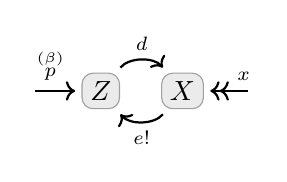
\begin{tikzpicture}[center base]
			\node[dpad0] (Z) {$Z$};
			\node[dpad0,right=.5 of Z] (X) {$X$};
			\draw[arr2, ->] (X) to[bend left=50]
				node[below]{$\scriptstyle e!$} (Z);
			\draw[arr2, ->] (Z) to[bend left=50]
				node[above]{$\scriptstyle d$} (X);
			\draw[arr2, <<-] (X) --
			  	node[above,pos=0.8]{$\scriptstyle x$}
			 	++(0.9, 0);
			\draw[arr2, <-] (Z) --
				node[above,pos=0.6]{$\scriptstyle \overset{(\beta)}p$}
				++(-0.9, 0);%
		\end{tikzpicture}}
	\]
\end{prop}
\begin{proof}
	\begin{align*}
		\aar*{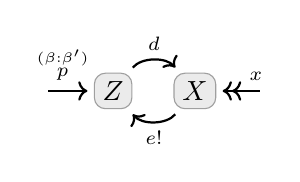
\begin{tikzpicture}[center base]
			\node[dpad0] (Z) {$Z$};
			\node[dpad0,right=.5 of Z] (X) {$X$};
			\draw[arr2, ->] (X) to[bend left=50]
			   node[below]{$\scriptstyle e!$} (Z);
			\draw[arr2, ->] (Z) to[bend left=50]
			   node[above]{$\scriptstyle d$} (X);
			\draw[arr2, <<-] (X) --
			   node[above,pos=0.8]{$\scriptstyle x$}
			   ++(0.9, 0);
			\draw[arr2, <-] (Z) --
			   node[above,pos=0.6]{$\scriptstyle \overset{(\beta : \beta')}p$}
			   ++(-0.9, 0);%
	   \end{tikzpicture}}
	   	&= \inf_\mu \bbr[\Bigg]{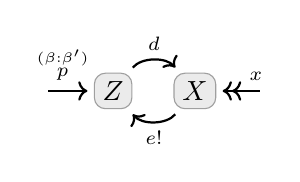
\begin{tikzpicture}[center base]
 		   \node[dpad0] (Z) {$Z$};
 		   \node[dpad0,right=.5 of Z] (X) {$X$};
 		   \draw[arr2, ->] (X) to[bend left=50]
 			   node[below]{$\scriptstyle e!$} (Z);
 		   \draw[arr2, ->] (Z) to[bend left=50]
 			   node[above]{$\scriptstyle d$} (X);
 		   \draw[arr2, <<-] (X) --
 			   node[above,pos=0.8]{$\scriptstyle x$}
 			   ++(0.9, 0);
 		   \draw[arr2, <-] (Z) --
 			   node[above,pos=0.6]{$\scriptstyle \overset{(\beta : \beta')}p$}
 			   ++(-0.9, 0);%
 	   \end{tikzpicture}}(\mu) \\
	   &= \inf_\mu \Ex_{\mu(X,Z)} \left[ \beta \log \frac{\mu(Z)}{p(Z)} + \log \frac{\mu(X,  Z)}{\mu(Z) d(X \mid Z)} \right] \\
   \intertext{As before, the only candidate for a joint distribution with finite score is $\delta_x(X) e(Z \mid X)$. Note that the marginal on $Z$ for this distribution is itself, since $\int_x \delta_x(X) e(Z \mid X)\;\mathrm dx = e(Z \mid x)$. Thus, our equation becomes}
	   &= \Ex_{\delta_x(X) e(Z \mid X)} \left[ \beta \log \frac{e(Z \mid x)}{p(z)} + \log \frac{\delta_x(X) e(Z \mid X)}{e(Z \mid x) d(x \mid Z)} \right] \\
	   &= \Ex_{e(Z \mid x)} \left[ \beta \log \frac{e(Z \mid x)}{p(Z)} + \log \frac{1}{ d(x \mid Z)} \right]
	   \qquad = -\beta\text{-}\mathrm{ELBO}_{p,e,d}(x).
	\end{align*}
\end{proof}

\section{Discussion}

\textbf{Inconsistency, in a different light.}
Nobody likes building broken things, and so those of who build systems commonly try to eliminate it in models by design. But in doing so, we unwittingly sacrifice tools for dealing with it if (and when) it does arise.


\textbf{A Universal Objective.}
Objective functions in machine learning are often quite opaque to new-comers.
Only a few of them are especially common, and they are often presented in an ad-hoc way; there are many loss functions that have the properties we need to train networks. So why do we lean so heavily on a few select choices (dependent on the problem setup), such as the cross entropy, and the ELBO objective?
PDGs provide one answer to this question.

There is perhaps a more important argument for using PDGs over other models. By designing a model, rather than an objective function, it is easier to understand what the pieces are, what is and is not relevant to the task, and no longer possible to twiddle with the objective until you get the results you want --- you can only twiddle with the model, where hacks are more easily spotted.

\textbf{Semantics for ``Graphical Models''.}
Often, autoencoder tutorials will include diagrams, and falsely claim that they are standard ``graphical models''. In these cases, among others, people are already reasoning about local probabilistic information in a graph. We have shown here that PDG semantics can sense of these informal diagrams in a way that is deeply connected with the variational reasoning involed.

\bibliographystyle{plain}
\bibliography{references}
\end{document}
